\documentclass[serif,dvipdfmx,10pt]{beamer}

% \usetheme{default}
% \usetheme{CambridgeUS}
% \usetheme{Madrid}
% \usetheme{metropolis}
\usetheme{Boadilla}
% \usetheme[numbering=fraction,block=fill,progressbar=frametitle]{metropolis}
\usepackage{bxdpx-beamer}
\usepackage{pxjahyper}
% \usepackage{colourchange}
\usepackage{minijs}
\usepackage{float}
\usepackage{tabu}
\usepackage{wrapfig}
\usepackage{amsfonts}
\usepackage{ascmac}
\usepackage{mathtools}
\usepackage{here}
\usepackage{listings}
\usepackage{mathrsfs}
\usepackage{caption}
\usepackage{bm}
\usepackage{multirow}
\usepackage{colortbl}
\usepackage{xcolor}
% \usepackage{algorithm2e}
\usepackage{algpseudocode}
\usepackage{arydshln}
\usepackage{tcolorbox}
\tcbuselibrary{listings,breakable,theorems,skins}
\usefonttheme{professionalfonts}
\usepackage{appendixnumberbeamer}

\usepackage{mathpazo}

% Set the title and author
\title[Coupled Phase-Oscillator Models]{Theoretical and Experimental Research\\on Coupled Phase-Oscillator Models}
\author{米田亮介}

% Set the date
\date{2023年2月24日}

% Set the logo and university
% \logo{
\includegraphics[width=1cm]{figs/logo.pdf}}
\titlegraphic{
    
\includegraphics[width=2cm]{figs/logo.pdf}
}
\institute[京大]{京都大学大学院情報学研究科先端数理科学専攻}

% Set the font and color theme
% \usefonttheme{professionalfonts}
% \usecolortheme{dolphin}

\setbeamertemplate{navigation symbols}{}

% \AtBeginSection[]{
%   \frame{\tableofcontents[currentsection, hideallsubsections]} %目次スライド
% }

\definecolor{forestgreen}{RGB}{34, 139, 34}
\definecolor{salmon}{RGB}{250, 128, 114}
\definecolor{deepskyblue}{RGB}{0, 191, 255}
\definecolor{lightgray}{RGB}{211, 211, 211}

\newcommand{\Kc}{K_{\mathrm{c}}}
\newcommand{\red}[1]{\textcolor{red}{#1}}
\newcommand{\blue}[1]{\textcolor{blue}{#1}}
\newcommand{\green}[1]{\textcolor{green}{#1}}
\newcommand{\gray}[1]{\textcolor{gray}{#1}}
\newcommand{\lightgray}[1]{\textcolor{lightgray}{#1}}
\newcommand{\gcheck}{\green{\checkmark}}
\newcommand{\diff}{\mathrm{d}}
\newcommand{\redbox}[2]{\tcboxmath[enhanced, frame hidden, colback=red!10, overlay={\node[below,red] at (frame.south) {#2};}]{#1}}
\newcommand{\greenbox}[2]{\tcboxmath[enhanced, frame hidden, colback=green!10, overlay={\node[below,black] at (frame.south) {#2};}]{#1}}


\begin{document}

% Title slide
\begin{frame}
  \titlepage
\end{frame}

\section{Introduction}
\begin{frame}{同期現象}
  \begin{itemize}
    \item 振動子が相互作用を通して振動のタイミングを揃える現象
    \begin{itemize}
      \item ホタルの発光
      \item メトロノーム
      \item ニューロンの発火、etc.
    \end{itemize}
  \begin{figure}
    \includegraphics[height=0.2\textheight]{figs/sync_image.pdf}
  \end{figure}
%   \item ホイヘンスが振り子時計の振り子の運動が揃うことに気づいたことが最初
  \item 悪い側面も
  \begin{itemize}
    \item ミレニアム橋の崩壊
    \item てんかん発作
  \end{itemize}
  \begin{figure}
    \includegraphics[height=0.2\textheight]{figs/sync_bad.pdf}
  \end{figure}
  \end{itemize}
\end{frame}

\begin{frame}{結合位相振動子系}
\begin{figure}
  \centering
  \includegraphics[width=\textwidth]{figs/phase_reduction.pdf}
\end{figure}
% \begin{block}{結合位相振動子系}
%   \centering
%   $\displaystyle \frac{\diff\theta_{i}}{\diff t}=\omega_{i}+\sum_{j=1}^{N}\Gamma_{ij}(\theta_{j}-\theta_{i})$
% \end{block}
\begin{align*}
  \frac{\diff\theta_{i}}{\diff t}=\redbox{\omega_{i}}{自然振動数}+\sum_{j=1}^{N}\redbox{\Gamma_{ij}(\theta_{i}-\theta_{j})}{結合関数}
\end{align*}
\begin{itemize}
  \item $\theta_{i}\in[0,2\pi)$: 各振動子の``位相''
  \item $\omega_{i}$: 各振動子が固有に持つ速度(自然振動数)
  \item $\Gamma_{ij}\colon\mathbb{S}^{1}\to\mathbb{R}$: 振動子間の\textbf{結合関数}
  \begin{itemize}
    \item 位相差$\theta_{j}-\theta_{i}$が入力
  \end{itemize}
\end{itemize}

\end{frame}

\begin{frame}{Questions}
\begin{itemize}
  \item \textbf{理論的側面} [Chapter 3, 4]
  \begin{figure}
    \centering
    \includegraphics[width=0.7\textwidth]{figs/theory_ponchi.pdf}
  \end{figure}
  \begin{itemize}
    \item 非同期状態から同期状態への転移の振る舞いは?
    \item どのような条件のもとで同期しやすい/同期しにくいのか?
  \end{itemize}
  \item \textbf{実験的側面} [Chapter 5]
  \begin{figure}
    \includegraphics[width=0.7\textwidth]{figs/gp_coupling_ponchi.pdf}
  \end{figure}
  \begin{itemize}
    \item 与えられたデータからどのようにモデルを推定するか?
  \end{itemize}
\end{itemize}
\end{frame}

% \begin{frame}{Outline}
% \begin{figure}
%     \centering
%     \includegraphics[width=\textwidth]{figs/phd_schematic.pdf}
% \end{figure}
% \end{frame}

\begin{frame}{博士論文の構成}
\begin{itemize}
  \item \lightgray{\textbf{Chapter 1}: イントロダクション}
  \item \lightgray{\textbf{Chapter 2}: 結合位相振動子系のレビュー}
  \item \textbf{Chapter 3}: Critical exponents in coupled phase-oscillator models on small-world networks
  \begin{itemize}
    \item Published in Physical Review E (2020)
  \end{itemize}
  \item \textbf{Chapter 4}: The lower bound of the network connectivity guaranteeing in-phase synchronization
  \begin{itemize}
    \item Published in Chaos (2021)
  \end{itemize}
  \item \textbf{Chapter 5}: Gaussian process regression approach to estimating phase dynamics from rhythmic data
  \begin{itemize}
    \item In preparation ...
  \end{itemize}
  \item \lightgray{\textbf{Chapter 6}: まとめ}
\end{itemize}
\end{frame}


\section{Critical exponents in coupled phase-oscillator models on small-world networks}
\begin{frame}{[\textbf{Chapter 3}] 結合位相振動子系}
  \begin{block}{大域結合位相振動子モデル}
  \centering
  $\displaystyle\frac{\diff\theta_{i}}{\diff t}=\omega_{i}+\frac{K}{N}\sum_{j=1}^{N}\Gamma(\theta_{j}-\theta_{i})$
  \begin{itemize}
    \item $\omega_{i}\sim g(\omega)$: \textbf{自然振動数分布$g(\omega)$からサンプル}
    \item $K$: 結合定数
    \item $\Gamma(\theta)$: 結合関数(周期$2\pi$)
  \end{itemize}
  \end{block}
  %どれほど同期しているかを表すパラメータ
  \checkmark \textbf{秩序変数}: 同期の強さを表すパラメータ
  \begin{align*}
    r=\left|\frac{1}{N}\sum_{j=1}^{N}e^{i\theta_{j}}\right|
  \end{align*}
  \begin{figure}
    \centering
    \includegraphics[width=0.4\textwidth]{figs/sync_notsync.pdf}
  \end{figure}
\end{frame}

\begin{frame}\frametitle{分岐図と臨界指数}
%  \begin{block}{臨界指数}
%  \begin{itemize}
%  \item もともと統計力学で研究されてきたもの
%  \item モデルの詳細には依存せず、普遍的な性質のみに依存すると考えられている。
%  \begin{itemize}
%    \item システムの次元
%    \item 相互作用の範囲
%  \end{itemize}
%  \end{itemize}
%  \end{block}
%  \begin{itemize}
%    \item 臨界点$\Kc$周りの立ち上がり
%    \begin{align*}
%      r\sim(K-\Kc)^{\beta}
%    \end{align*}
%    \item $\beta$: 臨界指数
%%    \item 臨界現象の背景には何らかの非自明な数理的構造があるとされている。
%%    \begin{itemize}
%%      \item 2次元Isingモデルの臨界現象の背景には\textbf{共形場理論}と呼ばれる数理的な構造がある。
%%      \item \textbf{Loewner微分方程式}とも関係があるらしい。
%%    \end{itemize}
%    \item $g(\omega)=\dfrac{\Delta}{\pi(\omega^{2}+\Delta^{2})}$(\textbf{Lorentz分布})のとき$\Kc=2\Delta$として
%    \begin{align*}
%      r=\sqrt{1-\frac{\Kc}{K}}\quad\Rightarrow\quad\beta=\frac{1}{2}
%    \end{align*}
%    \item 他の$g(\omega)$のときは??
%    \item 他の結合関数のときは??
%  \end{itemize}
  \begin{figure}
    \centering
    \includegraphics[scale=0.3]{figs/bif_exp-crop.pdf}
  \end{figure}
  \begin{itemize}
    \item $N\to\infty$での連続転移の臨界点近傍での立ち上がり: 臨界指数$\color{red}\beta$
    \begin{itemize}
      %\item 臨界指数は統計力学でよく研究され、\textbf{普遍性(universality)}を記述する
      \item 臨界指数は統計力学でよく研究されている
      \item 分布関数$g(\omega)$、結合関数$\Gamma(\theta)$による依存性
    \end{itemize}
  \end{itemize}
\end{frame}

%\begin{frame}\frametitle{分布関数$g(\omega)$と結合関数$\Gamma(\theta)$}
%  \begin{itemize}
%    \item 分布関数
%    \begin{align*}
%      g_{\color{red}n}(\omega)=\dfrac{n\Delta}{\Gamma(1/2n)}e^{-(\Delta\omega)^{2n}}
%    \end{align*}
%    \begin{itemize}
%      \item ${\color{red}n}=1$: ガウス分布
%      \item マクローリン展開: $g_{n}(\omega)=g_{n}(0)-C_{n}\omega^{\color{red}2n}+\cdots$
%    \end{itemize}
%    \begin{figure}
%      \centering
%      \includegraphics[scale=0.4]{gn.pdf}
%    \end{figure}
%    \item 結合関数
%    \begin{align*}
%      \Gamma(\theta)=\sin\theta+{\color{blue}a}\sin2\theta
%    \end{align*}
%    \begin{itemize}
%      \item ${\color{blue}a}=0$: 蔵本モデル
%%      \begin{align*}
%%        \frac{\diff\theta_{i}}{\diff t}=\omega_{i}+\frac{K}{N}\sum_{j=1}^{N}\sin(\theta_{j}-\theta_{i})
%%      \end{align*}
%    \end{itemize}
%  \end{itemize}
%\end{frame}

%\begin{frame}\frametitle{自然振動数分布の族}
%  \begin{align*}
%    &g^{(L)}_{n}(\omega)=\dfrac{n\sin(\pi/2n)}{\pi}\dfrac{\Delta^{2n-1}}{\omega^{2n}+\Delta^{2n}}\\
%    &g^{(G)}_{n}(\omega)=\dfrac{n\Delta}{\Gamma(1/2n)}e^{-(\Delta\omega)^{2n}}
%    \end{align*}
%    \begin{figure}
%    \centering
%    \includegraphics[scale=0.25]{figs/g_omega-crop.pdf}
%    \end{figure}
%    \begin{itemize}
%    \item Lorentz分布とGauss分布の一般化
%    \item $\omega=0$まわりの展開
%    \[
%    g_{n}(\omega)=g_{n}(0)-C_{n}\omega^{\red{2n}}+\cdots
%    \]
%    \item $\beta=\dfrac{1}{2n}$
%    \end{itemize}
%\end{frame}
%
%\begin{frame}\frametitle{$n=\infty$}
%  \begin{align*}
%    r-r_{\mathrm{c}}\propto(K-K_{\mathrm{c}})^{2/3}
%  \end{align*}
%  \begin{figure}
%    \begin{center}
%      \includegraphics[scale=0.3]{figs/bif-n-inf.pdf}
%    \end{center}
%  \end{figure}
%  \begin{itemize}
%    \item 臨界点でjumpが見られる
%    \item $\beta=\dfrac{2}{3}$
%  \end{itemize}
%\end{frame}
%
%\begin{frame}\frametitle{$\sin2\theta$を付け加える}
%  \begin{align*}
%    \frac{\diff\theta_{i}}{\diff t}=\omega_{i}+\frac{K}{N}\sum_{j=1}^{N}[\sin(\theta_{j}-\theta_{i})+\blue{a\sin2(\theta_{j}-\theta_{i})}]
%    \end{align*}
%    \begin{figure}
%    \includegraphics[scale=0.3]{figs/sin2-crop.pdf}
%    \end{figure}
%  \begin{itemize}
%%    \item \textbf{中心多様体縮約}を用いて$\beta=1$であることが示されている[Crawford 1995,Chiba 2011]。
%%    \begin{align*}
%%      &r\sim\frac{2(1-a)}{\Kc^{3}Ca}(K-\Kc)^{\red{1}}+\cdots\\
%%      &C=\mathcal{PV}\int_{\mathbb{R}}\diff\omega\frac{g'(\omega)}{\omega}
%%    \end{align*}
%    \item $a<0$で一山対称の$g(\omega)$のとき
%    \begin{align*}
%      \beta=1
%    \end{align*}
%  \end{itemize}
%\end{frame}

\begin{frame}\frametitle{臨界指数}
%  \begin{wrapfigure}[2]{R}[15pt]{0.5\textwidth}
%    \centering
%    \includegraphics[scale=0.3]{gn.pdf}
%  \end{wrapfigure}
%  \begin{align*}
%    &\Gamma(\theta)=\sin\theta+{\color{blue}a}\sin2\theta\\
%    &g_{n}(\omega)=\dfrac{n\Delta}{\Gamma(1/2n)}e^{-(\Delta\omega)^{2n}}=g_{n}(0)-C_{n}\omega^{\red{2n}}+\cdots
%  \end{align*}
\begin{columns}
  \begin{column}{0.36\linewidth}
    $\Gamma(\theta)=\sin\theta+{\color{blue}a}\sin2\theta$\\
    $g_{\color{red}n}(\omega)=\dfrac{ne^{-(\omega/\Delta)^{\color{red}2n}}}{\Gamma(1/2n)\Delta}$
  \end{column}
  \begin{column}{0.56\linewidth}
    \begin{figure}
      \centering
      \includegraphics[width=\linewidth]{figs/gn-crop.pdf}
    \end{figure}
  \end{column}
\end{columns}
  %$g_{n}(\omega)=\dfrac{n\Delta}{\Gamma(1/2n)}e^{-(\Delta\omega)^{2n}}=g_{n}(0)-C_{n}\omega^{\red{2n}}+\cdots$
  \begin{table}[htbp]
    \begin{center}
      \begin{tabular}{c||c|c|c}\hline\hline
       & \multicolumn{3}{c}{all-to-all} \\\hline
       & $a<0$ & $a=0$ & $a>0$ \\\hline\hline
      $n=1$ & \multirow{3}{*}{\begin{tabular}{c}$1$\\(Chiba 2011)\end{tabular}} & \begin{tabular}{c}$1/2$\\(Kuramoto 1975)\end{tabular} & \multirow{3}{*}{\begin{tabular}{c}(不連続)\\(Chiba 2011)\end{tabular}} \\\cline{3-3}
      $n\geq 2$ & & \begin{tabular}{c}$1/(2n)$\\(Basanarkov 2007)\end{tabular} & \\\cline{3-3}
      $n=\infty$ & &  \begin{tabular}{c}(不連続)\\(Pazo 2005)\end{tabular} &  \\\hline\hline
      \end{tabular}
    \end{center}
  \end{table}
  \begin{itemize}
    \item 理論的な導出はモデルの\textbf{全結合性}に強く依存
    \item 本研究: \underline{\textbf{現実に即したネットワークにおける臨界指数を調べる}}
  \end{itemize}
\end{frame}

%$1$\\[Chiba et al. 2011]}\end{tabular}

%\begin{frame}\frametitle{スモールワールドネットワーク}
%  \begin{itemize}
%    \item 現実のネットワークに関する研究
%    \begin{itemize}
%      \item ``6次の隔たり''
%      \item 強いクラスター化
%    \end{itemize}
%  \end{itemize}
%  \begin{block}{スモールワールド性}
%    \begin{itemize}
%      \item 平均ノード間距離$\langle l\rangle$がノード数$N$に対して$\langle l\rangle\ll N$
%      \item 平均クラスター係数がノード数$N$に依存しない
%    \end{itemize}
%  \end{block}
%  \begin{itemize}
%    \item \textbf{Watts-Strogatz model}: スモールワールド性を記述する代表的なモデル[Watts and Strogatz 1998]
%    \item \red{$O(N)$}本の枝を持つ(全結合グラフは$O(N^{2})$)
%  \end{itemize}
%  \begin{figure}
%    \includegraphics[width=8cm]{figs/mf_sw.pdf}
%  \end{figure}
%\end{frame}

%\begin{frame}\frametitle{Watts--Strogatz model}
%\begin{block}{アルゴリズム}
%  \begin{itemize}
%    \item[1] $N$個の頂点を持つ$k$-隣接グラフを生成する。
%    \item[2] $kN$本の枝のそれぞれに対して、確率$p$でエッジの一方(ランダムに選ぶ)の結合を切り離し、$N$頂点の中からランダムに選ばれた頂点につなぎ替える。
%    ただし、自己ループや多重エッジができないようにする。 
%  \end{itemize}
%\end{block}
%\begin{figure}
%  \begin{center}
%    \includegraphics[width=11cm]{figs/ring_sw.pdf}
%  \end{center}
%\end{figure}
%\end{frame}

\begin{frame}\frametitle{スモールワールドネットワーク}
  \begin{itemize}
    \item スモールワールドネットワーク
    \begin{itemize}
      \item ネットワーク全体の直径が小さい
    \end{itemize}
  %\begin{itemize}
    \item \textbf{Watts--Strogatz model}\footnote{Watts and Strogatz, 1998}: スモールワールド性を記述する代表的なモデル
    \begin{itemize}
      \item \red{$O(N)$}本の枝を持つ(全結合グラフは$O(N^{2})$)
    \end{itemize}
  \end{itemize}
  \vspace{2mm}
  \hspace{2.5cm}\textbf{全結合}\hspace{3cm}\textbf{スモールワールドネットワーク}
  \vspace{0.1mm}
  \begin{figure}
    \includegraphics[width=10cm]{figs/mf_sw-crop.pdf}
  \end{figure}
\end{frame}

\begin{frame}\frametitle{スモールワールドネットワーク上の結合振動子モデル}
  \begin{block}{スモールワールドネットワーク上の結合振動子モデル}
    \begin{center}
      $\displaystyle\frac{\diff\theta_{i}}{\diff t}=\omega_{i}+\frac{K}{2k}\sum_{j\in\Lambda_{i}}\left[\sin(\theta_{j}-\theta_{i})+a\sin2(\theta_{j}-\theta_{i})\right]$
    \end{center}
    \begin{itemize}
      \item $\Lambda_{i}$: $i$番目の振動子に接続する振動子のindex集合。Watts--Strogatzモデルに従って生成したネットワークによって定まる。
      \item $k$: (ネットワークの平均次数)/$2$
    \end{itemize}
  \end{block}
  \begin{table}[htbp]
    \begin{center}
      {\tabulinesep=1.2mm
      \begin{tabu}{c||c|c|c|c|c|c}\hline\hline
       & \multicolumn{3}{c|}{all-to-all($\color{red}O(N^{2})$)} & \multicolumn{3}{c}{small-world($\color{red}O(N)$)} \\\hline
       & $a<0$ & $a=0$ & $a>0$ & $a<0$ & $a=0$ & $a>0$\\\hline\hline
      $n=1$ & $1$ & $1/2$ & (不連続) & \red{?} & \begin{tabular}{c}(\red{$1/2$})\\(Hong 2001)\end{tabular} & \red{?}\\\hline
      $n\geq 2$ & $1$ & $1/(2n)$ & (不連続) & \red{?} & \red{?} & \red{?}\\\hline
      $n=\infty$ & $1$ & (不連続) & (不連続) & \red{?} & \red{?} & \red{?}\\\hline\hline
      \end{tabu}
      }
    \end{center}
  \end{table}
\end{frame}

%\begin{frame}\frametitle{臨界指数}
%  \begin{itemize}
%    \item 結合関数が$\sin\theta$で$g(\omega)$がGaussian($n=1$)の場合に数値的に臨界指数を求めている[Hong et al. 2002]。
%  \end{itemize}
%  \begin{table}[htbp]
%    \begin{center}
%      {\tabulinesep=1.2mm
%      \begin{tabu}{c||c|c|c|c|c|c}\hline\hline
%       & \multicolumn{3}{c|}{all-to-all} & \multicolumn{3}{c}{small-world} \\\hline
%       & $a<0$ & $a=0$ & $a>0$ & $a<0$ & $a=0$ & $a>0$\\\hline\hline
%      $n=1$ & $1$ & $\dfrac{1}{2}$ & (不連続) & ? & $\red{\dfrac{1}{2}}$ & ? \\\hline
%      $n\geq 2$ & $1$ & $\dfrac{1}{2n}$ & (不連続) & ? & ? & ? \\\hline
%      $n=\infty$ & $1$ & $\left(\dfrac{2}{3}\right)$ & (不連続) & ? & ? & ? \\\hline\hline
%      \end{tabu}
%      }
%    \end{center}
%  \end{table}
%  \begin{itemize}
%    \item 全結合蔵本モデルでは$g(\omega)$や結合関数によって多様な$\beta$が得られたが、スモールワールドネットワーク上の蔵本モデルでは$\beta$がどうなる??
%    \item まずは数値的に臨界指数を求める。
%  \end{itemize}
%\end{frame}

%\begin{frame}\frametitle{千葉論文との違い}
%  [Chiba et al. 2018]の中でスモールワールドネットワーク上の蔵本モデルの計算をしているが、
%  彼らは$k=\lfloor rN\rfloor, r\in(0,0.5)$としている。
%  \begin{figure}
%    \includegraphics[scale=0.15]{figs/graphon.pdf}
%  \end{figure}
%  \begin{itemize}
%    \item $r$の立ち上がりが
%    \begin{align*}
%      r\sim\frac{C}{\sqrt{-g''(0)}}(K-\Kc)^{1/2}+\cdots
%    \end{align*}
%    \item この設定だと$\beta$が$g(\omega)$に依存することを示唆している。(全結合と変わらない結果になりうる。)
%  \end{itemize}
%\end{frame}

\begin{frame}\frametitle{有限サイズスケーリング}
  \begin{block}{有限サイズスケーリング}
    \centering
      $\displaystyle r_{N}(K)N^{\beta/\bar{\nu}}=F((K-\Kc)N^{1/\bar{\nu}})$
  \end{block}
  \begin{itemize}
    \item 連続転移する系が臨界点近傍で\textbf{スケーリング関数}$F$に従う、という仮定
    \item 有限サイズ$N$のときの$r_{N}(K)$のデータをもとに$K_{\mathrm{c}},\red{\beta},\bar{\nu}$を推定
    \begin{itemize}
      \item Bayesian scaling analysis(ガウス過程回帰を用いる)によって推定\footnote{Harada 2011}
    \end{itemize}
    \item $a=0, n=1$
    \begin{figure}
      \centering
      \includegraphics[width=10cm]{figs/a-0_n-1_fss.pdf}
    \end{figure}
    %\begin{align*}
    %  \frac{\beta}{\bar{\nu}}=0.215\dots,\quad
    %  \frac{1}{\bar{\nu}}=0.405\dots\quad\Rightarrow\quad
    %  \beta=0.530\dots
    %\end{align*}
  \end{itemize}
\end{frame}

%\begin{frame}\frametitle{数値計算}
%  \begin{itemize}
%    \item システムサイズを$N=100$から$N=3200$まで計算
%    \item Watts-Strogatzモデル: $(k,p)=(3,0.2)$
%    \item $\{\theta_{i}\}$の初期条件: 円周上一様ランダム
%    \item $\{\omega_{i}\}$: $g_{n}^{(G)}(\omega)$に従うようにランダムにとる($n=1,2,3,\infty$それぞれについて計算)
%    \item 時間刻み幅$\diff t=0.1$で$t=500$まで(5000ステップ)4次のRunge-Kutta法で計算
%    \item 各システムサイズに対して100回から800回計算を行う
%    \item $r$は試行回数で平均をとったものを採用
%  \end{itemize}
%\end{frame}

%\begin{frame}\frametitle{数値計算結果}
%  \begin{block}{有限サイズスケーリング}
%    \begin{align*}
%      r=N^{-\beta/\bar{\nu}}F((K-\Kc)N^{1/\bar{\nu}})
%    \end{align*}
%  \end{block}
%  \begin{itemize}
%    \item $a=0,n=1$のとき
%  \begin{figure}
%    \includegraphics[width=10cm]{figs/a-0_n-1_fss.pdf}
%  \end{figure}
%  \begin{align*}
%    \frac{\beta}{\bar{\nu}}=0.2,\quad
%    \frac{1}{\bar{\nu}}=0.4\quad\Rightarrow\quad
%    \beta=0.5
%  \end{align*}
%\end{itemize}
%\end{frame}

%\begin{frame}\frametitle{数値計算結果($a=-0.2$)}
%  \begin{align*}
%    \frac{\beta}{\bar{\nu}}\approx 0.25,\quad
%    \frac{1}{\bar{\nu}}\approx 0.5\Rightarrow
%    \beta\approx \red{0.5}
%  \end{align*}
%  \begin{figure}
%    \includegraphics[width=10cm]{figs/bif-fss-sin2-a--02.pdf}
%  \end{figure}
%\end{frame}
%
%\begin{frame}\frametitle{数値計算結果($a=0.5$)}
%  \begin{align*}
%    \frac{\beta}{\bar{\nu}}\approx \red{0.15}
%  \end{align*}
%  \begin{figure}
%    \includegraphics[width=10cm]{figs/bif-fss-sin2-a-05.pdf}
%  \end{figure}
%\end{frame}

%\begin{frame}\frametitle{微分を使った計算}
%  \begin{align*}
%    &rN^{\beta/\bar{\nu}}=const.\\
%    &\frac{\diff r}{\diff K}|_{K=\Kc}N^{(\beta-1)/\bar{\nu}}=const.
%  \end{align*}
%  \begin{figure}
%    \begin{center}
%      \includegraphics[width=7cm]{figs/diff-test.pdf}
%    \end{center}
%  \end{figure}
%  \begin{itemize}
%    \item 傾き$\approx 0.19$
%    \item 先行研究とのずれ
%  \end{itemize}
%\end{frame}

\begin{frame}\frametitle{数値計算結果}
  \begin{align*}
    \Gamma(\theta)=\sin\theta+{\color{blue}a}\sin2\theta,\quad
    g_{\color{red}n}(\omega)=\dfrac{ne^{-(\omega/\Delta)^{\color{red}2n}}}{\Gamma(1/2n)\Delta}
  \end{align*}
  \begin{itemize}
    \item ${\color{blue}a}=0,-0.2,0.5$と$\red{n}=1,2,3,\infty$でそれぞれ臨界指数$\beta,\bar{\nu}$を計算
    \begin{table}[thbp]
      \begin{center}
        %{\tabulinesep=1.2mm
        \begin{tabu}{cc|cccc}\hline
          $\sin\theta+\blue{a}\sin2\theta$ & $g_{{\color{red}n}}(\omega)$ & $\beta$ & & $\bar{\nu}$ &\\\hline\hline
          \multirow{4}{*}{${\color{blue}a}=0$} & $\red{n}=1$ & $0.51(4)$ & \multirow{4}{*}{$\approx\red{\dfrac{1}{2}}$} & $2.40(6)$ & \multirow{4}{*}{$\approx\red{\dfrac{5}{2}}$}\\
           & $\red{n}=2$ & $0.49(2)$ & & $2.43(4)$ &\\
           & $\red{n}=3$ & $0.47(2)$ & & $2.46(4)$ &\\
           & $\red{n}=\infty$ & $0.46(2)$ & & $2.46(4)$ &\\\hline
           \multirow{4}{*}{${\color{blue}a}=-0.2$} & $\red{n}=1$ & $0.48(6)$ & \multirow{4}{*}{$\approx\red{\dfrac{1}{2}}$} & $2.36(8)$ & \multirow{4}{*}{$\approx\red{\dfrac{5}{2}}$}\\
           & $\red{n}=2$ & $0.51(4)$ & & $2.41(6)$ & \\
           & $\red{n}=3$ & $0.55(4)$ & & $2.50(6)$ &\\
           & $\red{n}=\infty$ & $0.49(4)$ & & $2.49(6)$ &\\\hline
        \end{tabu}
        %}
      \end{center}
    \end{table}
    % \item $n$によらず
    % \begin{align*}
    %   \beta\approx\frac{1}{2},\quad\bar{\nu}\approx\frac{5}{2}
    % \end{align*}
    % \item $a=0.5$では?
    \item $a=0.5$ではヒステリシスを確認$\Longrightarrow$\textbf{不連続転移}を示唆
  \end{itemize}
\end{frame}

\begin{frame}\frametitle{まとめと展望}
  \begin{align*}
    \Gamma(\theta)=\sin\theta+{\color{blue}a}\sin2\theta,\quad
    g_{\color{red}n}(\omega)=\dfrac{n}{\Gamma(1/2n)\Delta}e^{-(\omega/\Delta)^{\color{red}2n}}
  \end{align*}
  \begin{table}[htbp]
    \begin{center}
      {\tabulinesep=1.2mm
      \begin{tabu}{c||c|c|c|c|c|c}\hline\hline
        & \multicolumn{3}{c|}{all-to-all($\color{red}O(N^{2})$)} & \multicolumn{3}{c}{small-world($\color{red}O(N)$)} \\\hline
       & $a<0$ & $a=0$ & $0<a<1$ & $a=-0.2$ & $a=0$ & $a=0.5$\\\hline\hline
      $n=1$ & $1$ & $\dfrac{1}{2}$ & (不連続) & \red{$\dfrac{1}{2}$} & \red{$\dfrac{1}{2}$} & \red{(不連続)}\\\hline
      $n\geq 2$ & $1$ & $\dfrac{1}{2n}$ & (不連続) & \red{$\dfrac{1}{2}$} & \red{$\dfrac{1}{2}$} & \red{(不連続)}\\\hline
      $n=\infty$ & $1$ & (不連続) & (不連続) & \red{$\dfrac{1}{2}$} & \red{$\dfrac{1}{2}$} & \red{(不連続)}\\\hline\hline
      \end{tabu}
      }
    \end{center}
  \end{table}
  \begin{itemize}
    \item 全結合とスモールワールドネットワークで$\beta$が異なることがわかった。
    \begin{itemize}
      \item ノイズ系と同じ臨界指数
    \end{itemize}
    \item 理論的に臨界指数を求めたい。
    \begin{itemize}
      \item 連続極限をどう取る??(graphonを用いた解析はできない)
    \end{itemize}
  \end{itemize}
\end{frame}


\section{The lower bound of the network connectivity guaranteeing in-phase syn- chronization}
\begin{frame}{[\textbf{Chapter 4}] ネットワーク上の一様な結合振動子系}
  \begin{block}{ネットワーク上の一様な結合振動子系}
  \centering
  $\displaystyle\frac{\diff\theta_{i}}{\diff t}=\sum_{j\in[N]}a_{ij}\sin(\theta_{j}-\theta_{i})$
  \begin{itemize}
    \item $\theta_{i}\in[0,2\pi)$: $i$番目の振動子の位相
    \item $a_{ij}\in\{0,1\}$: ネットワークの隣接行列の$(i,j)$成分
  \end{itemize}
  \end{block}
  % \begin{figure}
  %     \centering
  %     \includegraphics[scale=0.3]{figs/graph_mat.pdf}
  % \end{figure}
  \begin{itemize}
    \item $\bm{\theta}_{0}=(0,0,\dots,0)^{\top}$: 完全同期解、すべての位相が同じ
    \item この解はネットワークによらずに\textbf{安定}
    \begin{itemize}
        \item 密であれば必ず同期すると期待(完全同期のみが安定平衡点)
        \item どれほど``密''であれば必ず同期する?
    \end{itemize}
  \end{itemize}
  \begin{figure}
    \centering
    \includegraphics[width=\textwidth]{figs/dense_sync_ponchi.pdf}
  \end{figure}
\end{frame}

% \begin{frame}{完全同期解}
%     \begin{block}{ネットワーク上の一様な結合振動子系}
%         \centering
%         $\displaystyle\frac{\diff\theta_{i}}{\diff t}=\sum_{j\in[N]}a_{ij}\sin(\theta_{j}-\theta_{i}),\ i\in[N]$
%         \begin{itemize}
%           \item $\theta_{i}\in[0,2\pi)$: $i$番目の振動子の位相
%           \item $a_{ij}\in\{0,1\}$: ネットワークの隣接行列の$(i,j)$成分
%         \end{itemize}
%     \end{block}
% \begin{itemize}
% \item $\bm{\theta}_{0}=(0,0,\dots,0)^{\mathsf{T}}$: 完全同期解、すべての位相が同じ
% \item この解はネットワークによらずに\textbf{安定}
% \begin{itemize}
%     \item $\bm{\theta}_{0}$まわりの線形安定性解析より従う
%     \item 勾配系であることからもわかる
%     \begin{align*}
%         \frac{\diff\bm{\theta}}{\diff t} = -\frac{\partial E(\bm{\theta})}{\partial\bm{\theta}},
%         \quad E(\bm{\theta}) = -\frac{1}{2}\sum_{i,j\in[N]}a_{ij}\cos(\theta_{j}-\theta_{i})
%     \end{align*}
% \end{itemize}
% \end{itemize}
% \end{frame}

\begin{frame}{接続数(connectivity)}
\begin{block}{connectivity $\mu$}
\centering
$\displaystyle\mu = \frac{\min_{i\in[N]}\sum_{j\in[N]}a_{ij}}{N-1}$
\end{block}
\begin{itemize}
    \item $\mu$はネットワークの``密具合''を表す
    \begin{itemize}
        \item ネットワークの最小次数を規格化したもの
        \item $\mu=1$のとき全結合ネットワーク
    \end{itemize}
\end{itemize}
\begin{figure}
    \centering
    \includegraphics[width=\textwidth]{figs/mu.pdf}
\end{figure}
\end{frame}

\begin{frame}{臨界接続数(critical connectivity)}
    \centering
  $\displaystyle\frac{\diff\theta_{i}}{\diff t}=\sum_{j\in[N]}a_{ij}\sin(\theta_{j}-\theta_{i})$
    \begin{table}[htb]
        \begin{tabular}{l||l}
            完全同期以外の安定平衡点が存在 & 完全同期のみが安定 \\
            (\blue{同期しない密なネットワーク}) & (\blue{必ず同期するネットワーク}) \\\hline
          $\mu\leq0.6809\dots$ (Wiley, 2006) & $\mu=1$ (Watanabe, 1994) \\
          $\mu\leq0.6818\dots$ (Canale, 2015) & $\mu\geq0.9395\dots$ (Taylor, 2012)\\
          $\mu\leq0.6828\dots$ (Townsend, 2020) & $\mu\geq0.7929\dots$ (Ling, 2019) \\
          \cellcolor[rgb]{1.0, 0.0, 0.0} & $\mu\geq0.7889\dots$ (Lu, 2020)
        \end{tabular}
      \end{table}
\begin{itemize}
    \item $\mu_{\mathrm{c}}$: 臨界接続数、完全同期解のみが安定平衡点となる$\mu$の境界
\begin{align*}
    0.6828\dots\leq\mu_{\mathrm{c}}\leq0.7889\dots
\end{align*}
\item 本研究: \underline{\textbf{できるだけ密な同期しないネットワークを探索する}}
\end{itemize}
\end{frame}

\begin{frame}{巡回グラフ}
\begin{itemize}
\item ネットワークとして巡回グラフを考える
\begin{itemize}
    \item 巡回グラフの対応する隣接行列は巡回行列
    \item $\bm{x}\in\{0,1\}^{N-1}$: 巡回行列を生成する列
    \begin{align*}
        a_{ij}=x_{i-j\bmod N},
        \quad x_{i}=x_{N-i}
    \end{align*}
    \item 強い対称性があるおかげで諸々の値の手計算が可能
\end{itemize}
\end{itemize}
\begin{figure}
    \centering
    \includegraphics[width=0.9\textwidth]{figs/circulant_graph_matrix.pdf}
\end{figure}
\end{frame}

\begin{frame}{$p$-twisted stateと線形固有値}
    \centering
  $\displaystyle\frac{\diff\theta_{i}}{\diff t}=\sum_{j\in[N]}a_{ij}\sin(\theta_{j}-\theta_{i})$
\begin{itemize}
\item ネットワークが巡回グラフの場合、$p$-twisted stateが平衡点
\begin{align*}
\bm{\theta}_{p}=\left(0,\frac{2\pi p}{N}, \frac{4\pi p}{N},\dots, \frac{2\pi (N-1)p}{N}\right)^{\top}\quad 0\leq p\leq\left\lfloor\frac{N}{2}\right\rfloor
\end{align*}
% \begin{itemize}
% \item $p=0$は完全同期解
% \end{itemize}
\begin{figure}
    \centering
    \includegraphics[width=0.8\textwidth]{figs/twisted_state.pdf}
\end{figure}
\item $p$-twisted stateまわりのJacobian行列の固有値$\bm{\lambda}$
\begin{align*}
    \lambda_{k}=\sum_{l\in[N-1]}x_{l}\cos\left(\frac{2\pi pl}{N}\right)\left[-1+\cos\left(\frac{2\pi kl}{N}\right)\right]
\end{align*}
% \begin{itemize}
%     \item $\lambda_{0}=0$: 系の大域的回転対称性より
%     \item $\lambda_{k},k=1,\dots,N-1$の正負が$p$-twisted stateの安定性を決める
% \end{itemize}
\end{itemize}
\end{frame}

\begin{frame}{方針}
\begin{itemize}
    \item 安定平衡点を持つネットワークを色々取り替える\\
    \begin{center}
        $\Downarrow$\\
    \end{center}
    その中で$\mu$が最大となるネットワークを選ぶ
    \item \textbf{最適化問題}による定式化
    \begin{itemize}
        \item $\bm{x}\in\{0,1\}^{N-1}$ $\Longrightarrow$ \textbf{整数計画問題}
        \item 制約条件
        \begin{itemize}
            \item $\lambda_{k}<0\Leftrightarrow L^{(N,p)}\bm{x}<\bm{0}$ (安定性)
            \[
                \left[L^{(N,p)}\right]_{kl} = \cos\left(\frac{2\pi pl}{N}\right)\left[-1+\cos\left(\frac{2\pi kl}{N}\right)\right]
            \]
            \item $x_{i}=x_{N-i} \Leftrightarrow C^{(N)}\bm{x}=0$ (無向グラフ)
            \[
                \left[C^{(N)}\right]_{kl}=\delta_{k,l}-\delta_{k,N-l}
            \]
        \end{itemize}
    \end{itemize}
\end{itemize}
\end{frame}

\begin{frame}{整数計画問題としての定式化}
``$N$体の振動子を持つ系において$p$-twisted stateが安定平衡点になるようなネットワークの中で最大のconnectivityはいくらか?''
\begin{block}{整数計画問題 $(N,p)$}
$N\geq2,1\leq p\leq\lfloor N/2\rfloor$に対して
\begin{align*}
\begin{split}
\textrm{maximize} & \quad\mu=\frac{1}{N-1}\bm{1}^{\top}\bm{x}, \\
\textrm{subject to} & \quad \bm{x}\in\left\{0,1\right\}^{N-1},\\
& \quad L^{(N,p)}\bm{x}<\bm{0},\quad \red{\mathrm{[stable]}}\\
& \quad C^{(N)}\bm{x} = \bm{0}.\quad \red{\mathrm{[undirected]}}
\end{split}
\end{align*}
\end{block}
\begin{itemize}
    \item $\mu^{(N,p)}$: 各$N,p$における整数計画問題の最大値
    % \item 実行可能解が存在しない場合: $\mu^{(N,p)}=-1$
\end{itemize}    
\end{frame}

% \begin{frame}{$\mu^{(N,p)}$の数値計算}
% \begin{itemize}
%     \item 最適化ライブラリ: \texttt{JuMP}(\texttt{Julia}), \texttt{pulp}(\texttt{Python})
% \end{itemize}
% \begin{figure}
%     \centering
%     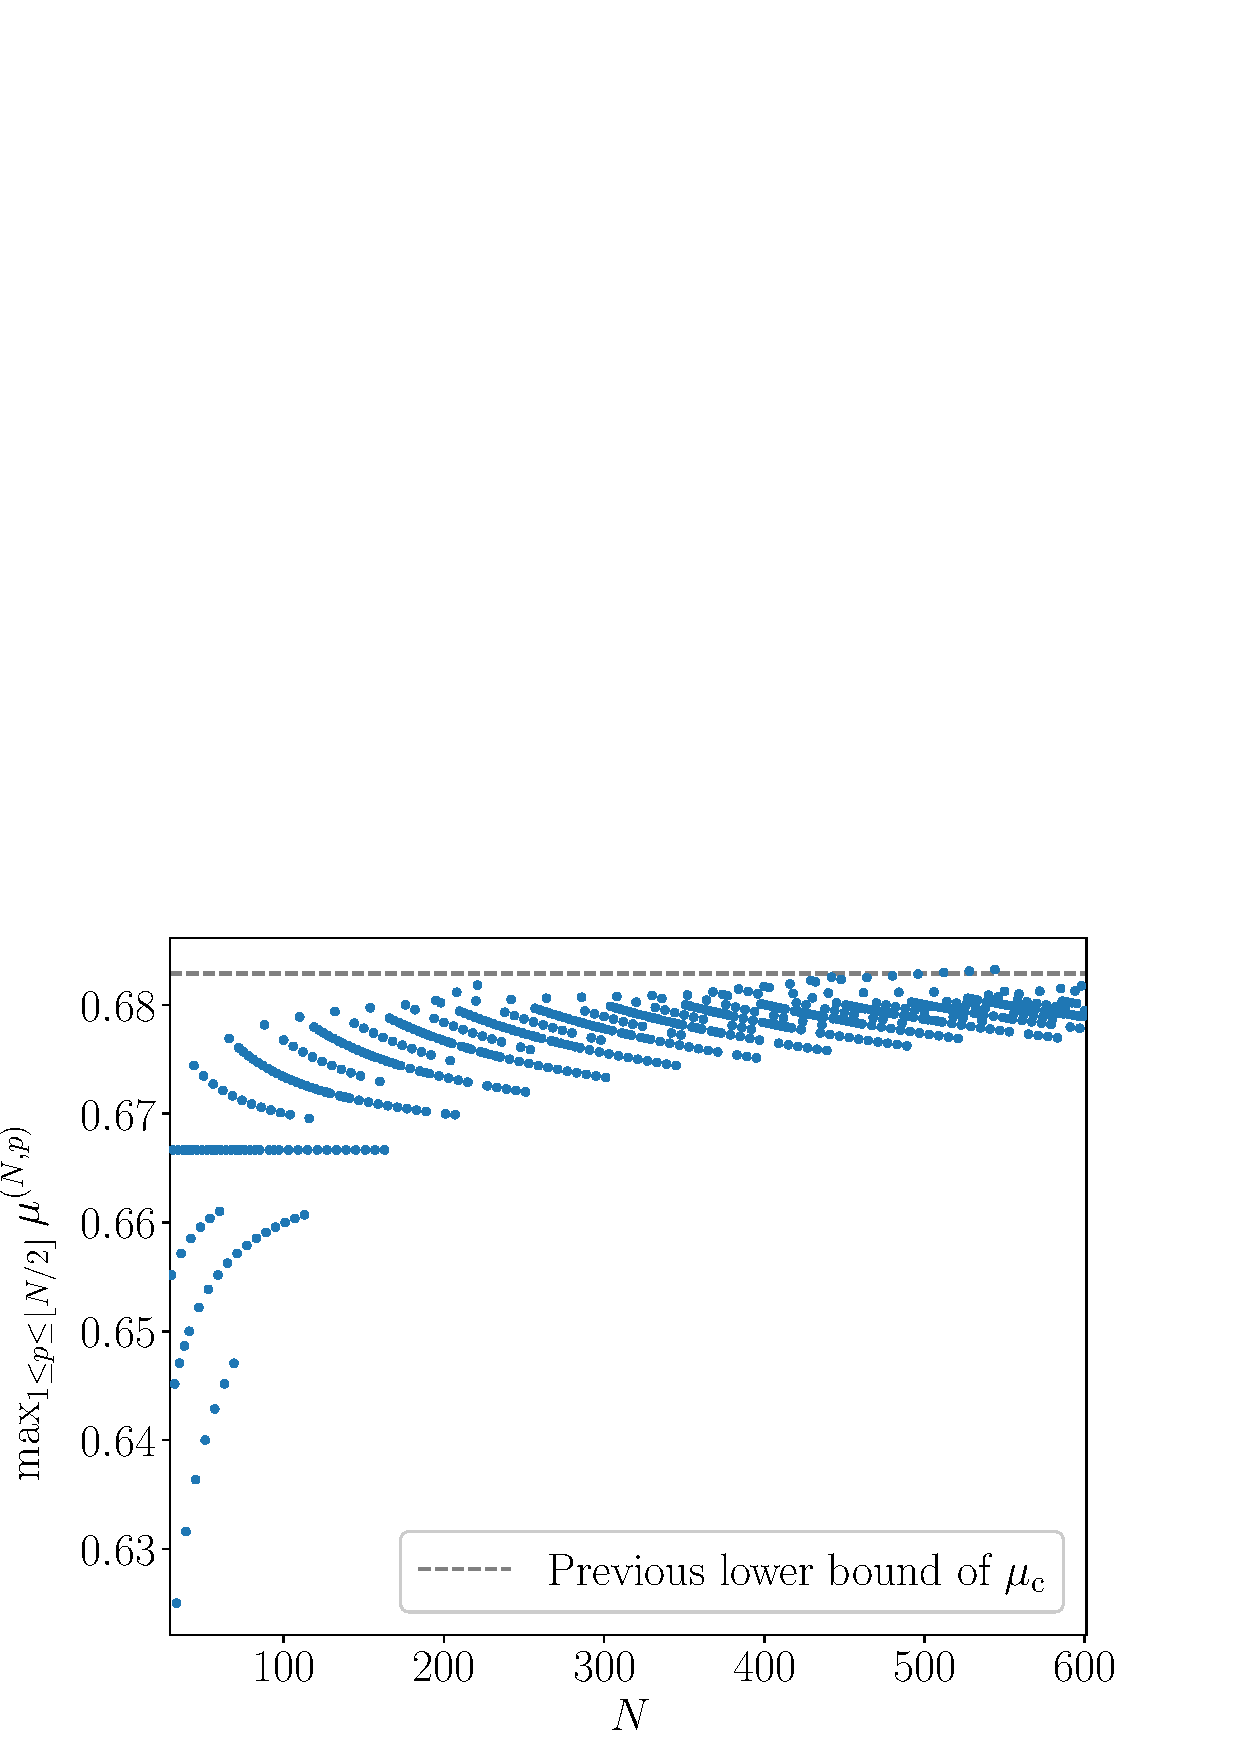
\includegraphics[width=0.9\textwidth]{figs/max_connect.pdf}
% \end{figure}
% \end{frame}

\begin{frame}{$\mu^{(N,p)}$の厳密解}
\begin{theorem}[$\mu^{(N,p)}$]
$N\geq2,1\leq p\leq\lfloor N/2\rfloor$に対して$m=\gcd(N,p),\widetilde{N}=N/m$とおく。
\begin{enumerate}
\item $\widetilde{N}=2,3,4$のとき実行可能解が存在しない。% $\mu^{(N,p)}=-1$
\item $\widetilde{N}\geq 5$のとき
\begin{align*}
    S_{k}^{(\widetilde{N})}=\sum_{l=1}^{k}\cos\left(\frac{2\pi l}{\widetilde{N}}\right)\left[-1+\cos\left(\frac{2\pi l}{\widetilde{N}}\right)\right]
\end{align*}
とし、$k_{\mathrm{c}}^{(\widetilde{N})}$を$S_{k}^{(\widetilde{N})}\geq0$なる最小の$k$と定義する。このとき、
\begin{align*}
    \mu^{(N,p)}=\frac{m(2k_{\mathrm{c}}-1)-1-2\lfloor mS_{k_{\mathrm{c}}-1}/(S_{k_{\mathrm{c}}}-S_{k_{\mathrm{c}}-1})\rfloor}{N-1}
\end{align*}
\end{enumerate}
\end{theorem}
\end{frame}

\begin{frame}{$\mu_{\mathrm{c}}$の下限}
\begin{theorem}[$\sup \mu^{(N,p)}$]
\begin{align*}
    &\sup\left\{\mu^{(N,p)} \mathrel{}\middle|\mathrel{} 1\leq p\leq \lfloor N/2\rfloor, N\geq2\right\}\\
    =&\lim_{m\to\infty}\mu^{(19m,m)}\\
    =&\frac{11}{19}-\frac{2}{19}\frac{\sum_{l=1}^{5}\left[-\cos\left(\frac{2\pi l}{19}\right)+\cos^{2}\left(\frac{2\pi l}{19}\right)\right]}{-\cos\left(\frac{12\pi}{19}\right)+\cos^{2}\left(\frac{12\pi}{19}\right)}=\red{0.683875\dots}
\end{align*}
\end{theorem}
\begin{itemize}
\item $\mu\leq 0.6838\dots$なるネットワークが存在して、完全同期解以外の安定平衡点が存在する。
\begin{align*}
    0.6838\dots\leq\mu_{\mathrm{c}}\leq0.7889\dots
\end{align*}
\end{itemize}
\end{frame}

\begin{frame}{まとめと展望}
    \centering
  $\displaystyle\frac{\diff\theta_{i}}{\diff t}=\sum_{j\in[N]}a_{ij}\sin(\theta_{j}-\theta_{i})$
    \begin{table}[htb]
        \begin{tabular}{l||l}
          完全同期以外の安定平衡点が存在 & 完全同期のみが安定 \\
          (\blue{同期しない密なネットワーク}) & (\blue{必ず同期するネットワーク}) \\\hline
          $\mu\leq0.6809\dots$ (Wiley, 2006) & $\mu=1$ (Watanabe, 1994) \\
          $\mu\leq0.6818\dots$ (Canale, 2015) & $\mu\geq0.9395\dots$ (Taylor, 2012)\\
          $\mu\leq0.6828\dots$ (Townsend, 2020) & $\mu\geq0.7929\dots$ (Ling, 2019) \\
          \red{$\mu\leq0.6838\dots$ (Yoneda, 2021)} & $\mu\geq0.7889\dots$ (Lu, 2020) \\ \hdashline \hdashline
          \green{$\mu\leq0.6875$ (Canale, 2022)} & \green{$\mu\geq0.75$ (Townsend, 2021)}
        \end{tabular}
      \end{table}
\begin{itemize}
    \item \textbf{$\mu_{\mathrm{c}}$の下からの評価について}
    \begin{itemize}
        \item 巡回グラフにおける他の平衡点? 他のネットワーク?
    \end{itemize}
\end{itemize}
\end{frame}


\section{Gaussian process regression approach to estimating phase dynamics from rhythmic data}

\begin{frame}{[\textbf{Chapter 5}] 結合関数推定}

\begin{figure}
  \centering
  \includegraphics[width=\textwidth]{figs/gp_coupling_ponchi.pdf}
\end{figure}

\begin{itemize}
  \item 先行研究: \textbf{ベイズ線形回帰} [Ota 2018]
  \begin{itemize}
    \item $\Gamma_{ij}$を有限次のFourier級数展開で近似し、Fourier係数を線形回帰
    \item 何次まで展開すべきかの自由度が残る
    \item Gibbs現象が生じる場合も
  \end{itemize}
  \item 本研究: \underline{\textbf{ガウス過程回帰を用いて結合関数を推定できるか?}}
  \begin{itemize}
    \item ``滑らかな周期関数''なる関数空間の中で回帰が可能になる
  \end{itemize}
\end{itemize}

\end{frame}

\begin{frame}{ガウス過程}
  \begin{block}{ガウス過程}
    確率過程$X_{t}$について、任意の組$(X_{t_{1}},\dots,X_{t_{k}})$が多次元正規分布に従うとき$X_{t}$を\textbf{ガウス過程}と呼ぶ
  \end{block}
  \begin{align*}
    f\sim\mathcal{GP}(m,k)
  \end{align*}
  \begin{itemize}
    \item $m(x)$: 平均関数
    \item $k(x,\tilde{x})$: カーネル関数
  \end{itemize}
  \begin{figure}
    \includegraphics[height=0.4\textheight]{figs/rbf_sample.pdf}
  \end{figure}
\end{frame}

\begin{frame}{カーネル関数}
ガウス過程で生成される関数の性質を決定(e.g. \textbf{滑らかさ}、\textbf{周期性}、\textbf{加法性})
\begin{figure}
  \includegraphics[width=0.6\textwidth]{figs/kernel_comparison.pdf}
\end{figure}
\begin{itemize}
  \item \textbf{additive model} $f(\bm{x})=\sum_{i}f_{i}(x_{i})$
  \begin{itemize}
    \item additiveなカーネルで生成 $k(\bm{x},\bm{\tilde{x}})=\sum_{i}k_{i}(x_{i},\tilde{x}_{i})$
  \end{itemize}
\end{itemize}
\begin{figure}
  \centering
  \includegraphics[width=0.5\textwidth]{figs/additive_gp.pdf}
\end{figure}
\end{frame}

\begin{frame}{ガウス過程回帰}
$y=f(x)$を満たすデータ$\mathcal{D}=\{(x_{i},y_{i})\}_{i}$によるガウス過程の事後分布で回帰\footnote{$[k_{XX}]_{ij}=k(x_{i},x_{j}),[k_{xX}]_{i}=k(x_{i},x),[\bm{y}]_{i}=y_{i},[m_{X}]_{i}=m(x_{i})$}
\begin{align*}
  &f\mid\mathcal{D}\sim\mathcal{GP}(\overline{m},\overline{k}),\\
  &\overline{m}(x)=m(x)+k_{xX}{k_{XX}}^{-1}(\bm{y}-m_{X}),\\
  &\overline{k}(x,\tilde{x})=k(x,\tilde{x})-k_{xX}{k_{XX}}^{-1}k_{X\tilde{x}}
\end{align*}
\begin{itemize}
  \item[\checkmark] \underline{ガウス過程のデータによる事後分布はまたガウス過程}
  \item[\checkmark] ハイパーパラメータは対数尤度最大化で最適化
  % \item[\checkmark] データ数$n$に対して$\mathcal{O}(n^{3})$の計算量が必要 $\Longrightarrow$ SVGPによる効率化
\end{itemize}
\begin{figure}
  \includegraphics[height=0.35\textheight]{figs/gpr_sample.pdf}
\end{figure}
\end{frame}

\begin{frame}{大規模データに対する処方箋}

  \begin{itemize}
    \item[\checkmark] データ数$n$に対して$\mathcal{O}(n^{3})$の計算量\\
    $\Longrightarrow$ 大規模データに対しては効率的な計算が必要
    \item \textbf{補助変数法(sparse GP)} [Quiñonero-Candela 2005]
    \begin{itemize}
      \item $m(<n)$個の補助入力点を用いて計算を効率化
    \end{itemize}
    \item \textbf{変分ベイズ法(SVGP)} [Hensman 2013]
    \begin{itemize}
      \item $m(<n)$個の補助入力点を用意
      \item 変分事後分布を学習し真の事後分布に近似
      \item データをサイズ$b$のミニバッチにわけることで学習を効率化
    \end{itemize}
  \end{itemize}
  
  \begin{table}[H]
    \caption*{計算量の比較}
    \begin{tabular}{l|cc>{\columncolor[rgb]{1.0,1.0,0.7}}c}
      & GP & sparse GP & SVGP \\\hline\hline
     推論コスト & $\mathcal{O}(n^{3})$ & $\mathcal{O}(nm^{2})$ & $\mathcal{O}(bm^{2}+m^{3})$ \\
     メモリコスト & $\mathcal{O}(n^{2})$ & $\mathcal{O}(nm)$ & $\mathcal{O}(bm+m^{2})$ \\
    \end{tabular}
  \end{table}
  
  \begin{itemize}
    \item 本研究ではSVGPを用いる
  \end{itemize}
\end{frame}

% \begin{frame}{アルゴリズム}
% \begin{columns}[t]
%   \begin{column}{0.4\textwidth}
%     \begin{enumerate}
%       \item 時系列の観測 ($N$体)
%       \item 位相への変換
%       \item $i$体目のベクトル場について
%       \begin{enumerate}
%         \item ベクトル場のデータ$\mathcal{D}_{i}$を生成
%         \begin{align*}
%           \mathcal{D}_{i}=\{(\bm{x}_{k},y_{k})\}_{k=1}^{n}
%         \end{align*}
%         \item SVGPで結合関数を推定
%       \end{enumerate}
%     \end{enumerate}
%   \end{column}
%   \begin{column}{0.6\textwidth}
%     \begin{itemize}
%       \item 時系列データの位相への変換
%       \begin{itemize}
%         \item 偏角もしくはヒルベルト変換
%         \item Kralemannの方法\footnote{Kralemann 2007}
%       \end{itemize}
%       \item ガウス過程回帰に用いるカーネル関数
%       \begin{align*}
%         k(\bm{x},\tilde{\bm{x}})=\sum_{j=1}^{N-1}\theta_{0}^{(j)}\exp(\theta_{1}^{(j)}\cos(x_{j}-\tilde{x}_{j}))
%       \end{align*}
%       \begin{itemize}
%         \item $N-1$変数のadditive modelへ回帰
%         \begin{align*}
%           \mathrm{input}:&\  \{\red{\theta_{j}-\theta_{i}}\}_{j\ne i}\\
%           \mathrm{output}:&\  \omega_{i}+\sum_{j\ne i}\Gamma_{ij}(\red{\theta_{j}-\theta_{i}})\\
%           \mathrm{target}:&\ \frac{\diff\theta_{i}}{\diff t}\simeq\frac{\theta_{i}(t_{k+1})-\theta_{i}(t_{k})}{t_{k+1}-t_{k}}
%         \end{align*}
%       \end{itemize}
%     \end{itemize}
%   \end{column}
% \end{columns}
% \end{frame}

\begin{frame}[t]{[提案手法] 観測・位相へ変換}
\begin{figure}
  \centering
  \includegraphics[width=\textwidth]{figs/flowchart1.pdf}
\end{figure}
\begin{figure}
  \centering
  \includegraphics[width=0.7\textwidth]{figs/observe_ponchi.pdf}
\end{figure}
\begin{figure}
  \centering
  \includegraphics[width=\textwidth]{figs/flowchart2.pdf}
\end{figure}
\begin{itemize}
  \item Kralemannの方法 [Kralemann 2007]
\end{itemize}
\begin{figure}
  \centering
  \includegraphics[width=\textwidth]{figs/data_to_phase.pdf}
\end{figure}
\end{frame}


\begin{frame}[t]{[提案手法] 結合関数推定}
  \begin{figure}
    \centering
    \includegraphics[width=\textwidth]{figs/flowchart3.pdf}
  \end{figure}
  \begin{columns}[t]
    \begin{column}{0.45\textwidth}
      $i$体目のベクトル場について\\
      \checkmark 回帰する関数 $\red{\Gamma_{ij}}\colon\mathbb{S}^{1}\to\mathbb{R}$
      \begin{align*}
        \frac{\diff\theta_{i}}{\diff t}=\sum_{j\ne i}\red{\Gamma_{ij}}(\theta_{j}-\theta_{i})
      \end{align*}
      \checkmark データ$\mathcal{D}_{i}=\{(\bm{x}_{k},y_{k})\}_{k}$
      \begin{align*}
        &\bm{x}_{k}=\begin{bmatrix}
          \theta_{1}(t_{k}) - \theta_{i}(t_{k})\\
          \vdots\\
          \theta_{N}(t_{k}) - \theta_{i}(t_{k})
        \end{bmatrix} \in \mathbb{T}^{N-1}\\
        &y_{k}=\frac{\theta_{i}(t_{k+1}) - \theta_{i}(t_{k})}{t_{k+1} - t_{k}} \in \mathbb{R}
      \end{align*}
    \end{column}
    \begin{column}{0.55\textwidth}
      \checkmark additiveな周期カーネル
      \begin{align*}
        &k(\bm{x},\tilde{\bm{x}})=\sum_{j\ne i}k_{j}(x_{j},\tilde{x}_{j})\\
        &k_{j}(x,\tilde{x})=p_{0}^{(j)}\exp(p_{1}^{(j)}\cos(x-\tilde{x}))
      \end{align*}
      \checkmark SVGPで結合関数を推定
      \begin{align*}
        \red{\Gamma_{ij}\mid\mathcal{D}_{i}}&\sim\mathcal{GP}(\overline{m}_{j}, \overline{k}_{j})\\
        \overline{m}_{j}(x)&=k_{j}(x,X)k(X,X)^{-1}\bm{y}\\
        \overline{k}_{j}(x,\tilde{x})&=k_{j}(x,\tilde{x})\\
        &\quad -k_{j}(x,X)k(X,X)^{-1}k_{j}(X,\tilde{x})
      \end{align*}
    \end{column}
  \end{columns}
\end{frame}

\begin{frame}{van der Pol振動子}
\begin{figure}
  \includegraphics[height=0.35\textheight]{figs/vdp_schematic.pdf}
\end{figure}
\begin{figure}
  \includegraphics[width=\textwidth]{figs/exp01case01.pdf}
\end{figure}
\end{frame}

\begin{frame}{ベイズ線形回帰との比較}
  \begin{figure}
    \centering
    \includegraphics[width=\textwidth]{figs/vdp.pdf}
  \end{figure}
  \begin{itemize}
    \item ベイズ線形回帰はフーリエ級数を何次まで展開するかのモデル選択が必要
    \begin{itemize}
      \item 適切な次数選択に失敗している
    \end{itemize}
    \item ガウス過程回帰は``滑らかな周期関数''なる関数空間全体の中での回帰を行う
  \end{itemize}
\end{frame}

\begin{frame}{神経細胞モデル}
  \begin{columns}[t]
    \begin{column}{0.5\textwidth}
      \checkmark 興奮性・抑制性細胞によるネットワークモデル
      \begin{figure}
        \includegraphics[width=0.9\columnwidth]{figs/snn_netplot.pdf}
      \end{figure}
      \checkmark 観測時系列
      \begin{figure}
        \includegraphics[width=0.9\columnwidth]{figs/snn_volt.pdf}
      \end{figure}
    \end{column}
    \begin{column}{0.5\textwidth}
      \checkmark 結合関数の推定
      \begin{figure}
        \includegraphics[width=\columnwidth]{figs/snn_gp_100.pdf}
        \caption*{黒点線: 理論\ \red{赤線: $\mathcal{GP}$回帰}}
      \end{figure}
    \end{column}
  \end{columns}
\end{frame}

\begin{frame}{まとめと展望}
  \begin{itemize}
    \item ガウス過程回帰を用いてリズム現象が従う結合位相振動子系を推定
    \begin{align*}
      k(\bm{x},\tilde{\bm{x}})=\sum_{j=1}^{N-1}p_{0}^{(j)}\exp(p_{1}^{(j)}\cos(x_{j}-\tilde{x}_{j}))
    \end{align*}
    \begin{figure}
      \includegraphics[height=0.3\textheight]{figs/exp01case01.pdf}
    \end{figure}
    \item 離散のデータから微分を近似するため誤差が生じる
    \begin{itemize}
      \item \textbf{Neural SDE} [Li 2020]によるベクトル場の回帰の検討 %\footnote{Ricky T. Q. Chen 2018}
      \begin{align*}
        \diff x=f(t,x;\theta_{f})\diff t+g(t,x;\theta_{g})\diff W_{t}
      \end{align*}
      \item 解軌道の$\theta_{f},\theta_{g}$微分をadjoint方程式で求める手法
    \end{itemize}
  \end{itemize}
\end{frame}

\section{Conclusion}
\begin{frame}{Conclusion}
本研究: \underline{\textbf{同期現象を記述する数理モデルの研究}}

\begin{tcolorbox}[enhanced,
  colframe=deepskyblue,
  colback=deepskyblue!20!white,
  coltitle=black,
  drop fuzzy shadow,
  title=\textbf{結合位相振動子系}]
  \[\displaystyle \frac{\diff\theta_{i}}{\diff t}=\omega_{i}+\sum_{j\ne i}\Gamma_{ij}(\theta_{j}-\theta_{i})\]
\end{tcolorbox}

\begin{tcolorbox}[enhanced,
  colframe=forestgreen,
  colback=forestgreen!20!white,
  coltitle=black,
  drop fuzzy shadow,
  title=\textbf{理論的側面}]
\begin{itemize}
  \item \underline{\textbf{現実に即したネットワークにおける臨界指数を調べる}}\\
  $\Longrightarrow$ SWネットワークにおいて全結合と異なる臨界指数を取る
  \item \underline{\textbf{できるだけ密な同期しないネットワークを探索する}}\\
  $\Longrightarrow$ $\mu=0.6838\dots$なるネットワークを整数計画問題により発見
\end{itemize}
\end{tcolorbox}

\begin{tcolorbox}[enhanced,
  colframe=salmon,
  colback=salmon!20!white,
  coltitle=black,
  drop fuzzy shadow,
  title=\textbf{実験的側面}]
\begin{itemize}
  \item \underline{\textbf{ガウス過程回帰を用いて結合関数を推定できるか?}}\\
  $\Longrightarrow$ additiveな周期カーネルの提案
\end{itemize}
\end{tcolorbox}
\end{frame}

\appendix

\begin{frame}
    \centerline{\LARGE{APPENDIX}}
\end{frame}

\section{Bayesian Scaling Analysis}
\label{sec:bsa}
We briefly review the Bayesian scaling analysis~\cite{harada2011,harada2015},
 a statistical method for estimating the values such as $\beta, \bar{\nu},$ and $K_{\rm c}$ in Eq.~\eqref{eq:finite-size}.
We write these values as $\theta_{p}=(\beta,\bar{\nu},K_{\mathrm{c}})$.
We assume that the scaling function $F$ in Eq.~\eqref{eq:finite-size} obeys a Gaussian process
\begin{align}
    F\sim\mathcal{GP}(m,k_{\theta_{h}}),
\end{align}
with mean function $m(\cdot)$ and covariance kernel $k_{\theta_{h}}(\cdot,\cdot)$.
Here $\theta_{h}$ denotes the hyperparameters of covariance kernel.
We also set $m=0$ for simplicity.
In the following, we also use the notation $\bm{\theta}=(\theta_{h},\theta_{p})$.
For the data $\{r_{N_{i}}(K_{i})\}_{i=1}^{M}$,
the rescaled data $X_{\theta_{p},i}=(K_{i}-K_{\mathrm{c}})N_{i}^{1/\bar{\nu}}$
and $Y_{\theta_{p},i}=r_{N_{i}}(K_{i})N_{i}^{\beta/\bar{\nu}}$
must collapse on the scaling function as $Y_{\theta_{p},i}=F(X_{\theta_{p},i})$.
Since $F$ is a Gaussian process, $Y_{\theta_{p}}$ obeys a $M$-dimensional
Gaussian distribution, and the probability of $Y$ for the parameter $\bm{\theta}$ is
\begin{align}
    &p(Y\mid\bm{\theta})=\mathcal{N}(Y_{\theta_{p}}\mid\bm{0},K_{\bm{\theta}})\notag\\
    =&\frac{1}{(2\pi)^{N/2}[\det K_{\bm{\theta}}]^{1/2}}
    \exp\left[-\frac{1}{2}Y_{\theta_{p}}^{\mathsf{T}}K_{\bm{\theta}}^{-1}Y_{\theta_{p}}\right].
    \label{eq:posterior}
\end{align}
Here, $[K_{\bm{\theta}}]=k_{\theta_{h}}(X_{\theta_{p},i},X_{\theta_{p},j})$ is $M\times M$ dimensional matrix.
By assuming that the prior distribution of $\bm{\theta}$ is uniform, we have
\begin{align}
    p(\bm{\theta}\mid Y)\propto p(Y\mid\bm{\theta}),
\end{align}
from Bayes' theorem.
The most probable parameters $\bm{\theta}$ are, therefore,  estimated by finding the minimum of likelihood function given by
\begin{align}
  L_{\bm{\theta}}
%  = \log|K_{\bm{\theta}}|
  = \log(\det K_{\bm{\theta}})
  + Y_{\theta_{p}}^{\mathsf{T}}K_{\bm{\theta}}^{-1}Y_{\theta_{p}},
    \label{eq:likelihood}
\end{align}
which is obtained by taking $\log$ and discarding constants in Eq.~\eqref{eq:posterior}.
The gradient of $L_{\bm{\theta}}$ for an element $\theta\in\bm{\theta}$ is given by
\begin{equation}
\begin{split}
    \frac{\partial L_{\bm{\theta}}}{\partial \theta}
    =&\mathrm{tr}\left[K_{\bm{\theta}}^{-1}\frac{\partial K_{\bm{\theta}}}{\partial\theta}\right]-(K_{\bm{\theta}}^{-1}Y_{\theta_{p}})^{\mathsf{T}}\frac{\partial K_{\bm{\theta}}}{\partial \theta}(K_{\bm{\theta}}^{-1}Y_{\theta_{p}})\\
    &+2Y_{\theta_{p}}^{\mathsf{T}}K_{\bm{\theta}}^{-1}\frac{\partial Y_{\theta_{p}}}{\partial\theta},
\end{split}
\end{equation}
and using this gradient, the gradient method gives us the most probable parameters $\bm{\theta}$.

In this paper, we consider a kernel based on a radial basis function (RBF) kernel
\begin{align}
    k_{\theta_{h}}(x,y)=\theta_{1}\exp\left[-\frac{(x-y)^{2}}{\theta_{2}}\right]+\theta_{3}\delta(x,y),
\end{align}
which is parameterized by $\theta_{h}=(\theta_1,\theta_2,\theta_3)$ with $\theta_{1,2,3}>0$,
and $\delta(x,y)=1$ when $x=y$, otherwise $\delta(x,y)=0$.
Here, $\theta_{3}$ denotes the data fidelity.
Roughly speaking, a sample path of Gaussian process associated with a RBF kernel are known to be an infinitely differentiable function;
see \cite[Corollary~4.13]{kanagawa2018} for a rigorous statement.
Therefore, the Bayesian scaling analysis only assumes the smoothness of a scaling function,
and it does not need an explicit form.
See the reference \cite{harada2011,harada2015} for more detailed discussions.



\end{document}
